\documentclass[11pt]{article}

\usepackage[a4paper]{geometry}
\geometry{left=2.0cm,right=2.0cm,top=2.5cm,bottom=2.5cm}

\usepackage{ctex} % 支持中文的LaTeX宏包
\usepackage{amsmath,amsfonts,graphicx,amssymb,bm,amsthm,mathrsfs,mathtools,breqn} % 数学公式和符号的宏包集合
\usepackage{algorithm,algorithmicx} % 算法和伪代码
\usepackage[noend]{algpseudocode} % 算法和伪代码
\usepackage{fancyhdr} % 自定义页眉页脚
\usepackage[framemethod=TikZ]{mdframed} % 创建带边框的框架
\usepackage{fontspec} % 字体设置
\usepackage{adjustbox} % 调整盒子大小
\usepackage{fontsize} % 设置字体大小
\usepackage{tikz,xcolor} % 绘制图形和使用颜色
\usetikzlibrary{positioning}
\usepackage{multicol} % 多栏排版
\usepackage{multirow} % 表格中合并单元格
\usepackage{pdfpages} % 插入PDF文件
\usepackage{listings} % 在文档中插入源代码
\usepackage{wrapfig} % 文字绕排图片
\usepackage{bigstrut,multirow,rotating} % 支持在表格中使用特殊命令
\usepackage{booktabs} % 创建美观的表格
\usepackage{circuitikz} % 绘制电路图
\usepackage{zhnumber} % 中文序号(用于标题)
\usepackage{tabularx} % 表格折行
\usepackage{float} % 图片插入
\usepackage{longtable} % 长表格

\definecolor{dkgreen}{rgb}{0,0.6,0}
\definecolor{gray}{rgb}{0.5,0.5,0.5}
\definecolor{mauve}{rgb}{0.58,0,0.82}
\lstset{
  frame=tb,
  aboveskip=3mm,
  belowskip=3mm,
  showstringspaces=false,
  columns=fixed,
  framerule=1pt,
  rulecolor=\color{gray!35},
  backgroundcolor=\color{gray!5},
  basicstyle={\small\ttfamily},
  numbers=none,
  numberstyle=\tiny\color{gray},
  keywordstyle=\color{blue},
  commentstyle=\color{dkgreen},
  stringstyle=\color{mauve},
  breaklines=true,
  breakatwhitespace=true,
  tabsize=3,
}

% 轻松引用, 可以用\cref{}指令直接引用, 自动加前缀. 
% 例: 图片label为fig:1
% \cref{fig:1} => Figure.1
% \ref{fig:1}  => 1
\usepackage[capitalize]{cleveref}
% \crefname{section}{Sec.}{Secs.}
\Crefname{section}{Section}{Sections}
\Crefname{table}{Table}{Tables}
\crefname{table}{Table.}{Tabs.}

% \setmainfont{Palatino Linotype.ttf}
% \setCJKmainfont{SimHei.ttf}
% \setCJKsansfont{Songti.ttf}
% \setCJKmonofont{SimSun.ttf}
\punctstyle{kaiming}
% 偏好的几个字体, 可以根据需要自行加入字体ttf文件并调用

\renewcommand{\emph}[1]{\begin{kaishu}#1\end{kaishu}}

% 对 section 等环境的序号使用中文
\renewcommand \thesection{\zhnum{section}、}
\renewcommand \thesubsection{\arabic{subsection}}


%%%%%%%%%%%%%%%%%%%%%%%%%%%
%改这里可以修改实验报告表头的信息
\newcommand{\name}{陈琛、王荦璠、张钧玮}
\newcommand{\studentNum}{80}
\newcommand{\major}{计算机科学与技术}
\newcommand{\labNum}{7}
\newcommand{\labName}{高速缓存设计专题}
%%%%%%%%%%%%%%%%%%%%%%%%%%%

\begin{document}
\begin{center}
  \LARGE \bf 中国科学院大学 \\《计算机体系结构(研讨课)》实验报告
\end{center}

\begin{center}
  \emph{姓名} \underline{\makebox[12em][c]{\name}} 
  \emph{箱子号} \underline{\makebox[7em][c]{\studentNum}}
  \emph{专业} \underline{\makebox[15em][c]{\major}}\\
  \emph{实验项目编号} \underline{\makebox[3em][c]{\labNum}}
  \emph{实验名称} \underline{\makebox[30em][c]{\labName}}\\
\end{center}

\section{实验任务}

本次实验是高速缓存设计专题,包含四个递进式的实践任务。实验的总体目标是为CPU添加Cache支持,通过引入指令Cache和数据Cache来提升CPU的访存性能,同时保持对非缓存访问的正确处理能力。工作划分为四个阶段:首先设计独立的Cache模块,然后将Cache模块作为ICache集成到CPU中,接着将Cache模块作为DCache集成到CPU中,最后实现对Cache维护指令的支持。

\begin{itemize}
    \item \textbf{实践任务20:Cache模块设计}
    
    设计Cache模块,这是提升CPU访存性能的核心组件。Cache采用8KB容量、两路组相联的设计规格,采用LRU或伪随机替换算法。需要实现Look Up、Hit Write、Replace和Refill四种基本操作,设计主状态机和Write Buffer状态机来控制Cache的工作流程。完成后利用Cache模块级验证环境对所设计的Cache进行验证,通过仿真和上板验证。
    
    \item \textbf{实践任务21:在CPU中集成ICache}
    
    要求将实践任务20完成的Cache模块作为ICache集成到实践任务19完成的CPU中,修改IFU模块以支持Cache接口并正确处理Uncache访问,修改CPU中的AXI转换桥以支持Burst传输模式。完成后在采用AXI总线的SoC验证环境里完成exp21对应func的功能验证,要求成功通过仿真和上板验证。
    
    \item \textbf{实践任务22:在CPU中集成DCache}
    
    要求将实践任务20完成的Cache模块作为DCache集成到实践任务21完成的CPU中,修改MEMU模块以支持Cache接口,处理好数据访存与Cache的交互,确保Load/Store指令能够正确利用Cache提升性能。完成后在采用AXI总线的SoC验证环境里完成exp22对应func的功能验证,要求成功通过仿真和上板验证。
    
    \item \textbf{实践任务23:在CPU中添加CACOP指令}
    
    要求在CPU中增加CACOP指令的支持,用于Cache的初始化和维护操作。CACOP指令需要复用Cache模块已有的数据通路,实现对Cache行的Invalid、Store Tag、Hit Invalid等操作。完成后在采用AXI总线的SoC验证环境里完成exp23对应func的功能验证,要求成功通过仿真和上板验证。
\end{itemize}

\section{设计详细分析}

\subsection{Cache模块设计(exp20)}

exp20的目标是独立完成一个可复用的Cache模块,为后续在CPU中集成指令Cache和数据Cache打下基础。我们实现的Cache采用8KB容量、两路组相联的规格。为了在性能和实现复杂度之间取得平衡,选择了Tag和Data同步访问的VIPT(虚Index实Tag)方式,这样可以将TLB查找与Cache访问并行进行。Cache采用伪随机替换算法,通过线性反馈移位寄存器(LFSR)生成伪随机数来选择被替换的路。在写策略上,采用写回写分配(write-back write-allocate)策略,这样写操作在发生Cache缺失时的处理流程和读操作基本一致,能够简化控制逻辑的设计。

\subsubsection{Cache设计规格与地址划分}

根据教材的建议,我们的Cache模块采用如下设计规格:容量为8KB(每路4KB),两路组相联,Cache行大小为16B。这样的配置下,Index需要8位(256项),Offset需要4位(16字节),Tag需要20位。对Cache进行访问时,使用虚拟地址的[11:4]作为Index索引(这是VIPT的关键),使用物理地址的[31:12]作为Tag进行比较。在我们的设计中,每个Cache行包含Tag、Valid位、Dirty位和Data四部分信息。为了优化RAM的使用效率,我们将Tag和Valid位合并存储在一起(21位宽),Dirty位使用寄存器实现,Data部分则按4字节划分为4个Bank,每个Bank单独使用一个Block RAM实现。

Cache模块对外提供两组接口。第一组是与CPU流水线的交互接口,包括请求的有效信号、操作类型(读或写)、索引、标签、偏移、写字节使能、写数据和uncache标志等输入信号,以及地址传输完成信号(addr\_ok)、数据传输完成信号(data\_ok)和读数据等输出信号。第二组是与AXI总线接口模块的交互接口,包括读请求、写请求的各项控制信号和数据信号。这样的接口划分使得Cache模块能够很好地融入现有的CPU设计中,与流水线的握手机制保持一致,同时也便于后续集成时进行调试。

\subsubsection{Cache RAM的组织与实例化}

Cache模块内部的存储结构是整个设计的核心。我们将逻辑上的Cache表拆分成多个物理RAM,每一路包含一个TAGV RAM(256×21位,用于存储Tag和Valid位)、四个Data Bank RAM(每个256×32位,每个Bank对应Cache行中的一个字),以及用寄存器实现的Dirty表(256位)。在Cache模块中,定义了所有RAM的接口信号:

\begin{lstlisting}[language=Verilog]
// TAGV RAM interface signals
wire [ 7:0] tagv_addr;
wire [20:0] tagv_wdata;
wire [20:0] tagv_way0_rdata;
wire [20:0] tagv_way1_rdata;
wire        tagv_way0_en;
wire        tagv_way1_en;
wire        tagv_way0_we;
wire        tagv_way1_we;

// DATA Bank RAM interface signals
wire [ 7:0] data_addr;
wire [31:0] data_wdata;
wire [31:0] data_way0_bank0_rdata;
wire [31:0] data_way0_bank1_rdata;
wire [31:0] data_way0_bank2_rdata;
wire [31:0] data_way0_bank3_rdata;
// ... (Way1 Bank signals similar)
wire        data_way0_bank0_en;
// ... (other enable signals)
wire [ 3:0] data_way0_bank0_we;
// ... (other write enable signals with byte granularity)

// Dirty bit table (implemented using registers)
reg [255:0] dirty_way0;
reg [255:0] dirty_way1;
\end{lstlisting}

然后实例化所有的RAM模块。对于TAGV RAM,为每一路实例化一个:

\begin{lstlisting}[language=Verilog]
// TAGV RAM - Way 0
tagv_ram tagv_way0_inst (
    .clka   (clk),
    .ena    (tagv_way0_en),
    .wea    (tagv_way0_we),
    .addra  (tagv_addr),
    .dina   (tagv_wdata),
    .douta  (tagv_way0_rdata)
);

// TAGV RAM - Way 1
tagv_ram tagv_way1_inst (
    .clka   (clk),
    .ena    (tagv_way1_en),
    .wea    (tagv_way1_we),
    .addra  (tagv_addr),
    .dina   (tagv_wdata),
    .douta  (tagv_way1_rdata)
);
\end{lstlisting}

对于Data Bank RAM,每一路需要实例化4个Bank,总共8个RAM实例。每个Bank RAM配置为支持字节写使能,这样可以支持SB、SH等字节级写操作:

\begin{lstlisting}[language=Verilog]
// DATA Bank RAM - Way 0 Bank 0
data_bank_ram data_way0_bank0_inst (
    .clka   (clk),
    .ena    (data_way0_bank0_en),
    .wea    (data_way0_bank0_we),  // 4-bit byte write enable
    .addra  (data_addr),
    .dina   (data_wdata),
    .douta  (data_way0_bank0_rdata)
);
// ... (other 7 Bank RAM instances)
\end{lstlisting}

Dirty表使用寄存器数组实现,在复位时初始化为全0。这样的组织方式能够很好地映射到FPGA的Block RAM资源上,Tag和Data可以同步读取,满足单周期Cache命中的需求。

\subsubsection{主状态机与Write Buffer状态机}

Cache模块的控制逻辑由两个状态机协同工作。主状态机负责处理Cache查找、缺失、替换和填充的整个流程,而Write Buffer状态机专门处理写命中情况下的写入操作。状态机的状态编码采用one-hot编码方式以提高状态转换的速度:

\begin{lstlisting}[language=Verilog]
// Main state machine states
localparam STATE_IDLE    = 5'b00001;
localparam STATE_LOOKUP  = 5'b00010;
localparam STATE_MISS    = 5'b00100;
localparam STATE_REPLACE = 5'b01000;
localparam STATE_REFILL  = 5'b10000;

// Write Buffer state machine states
localparam WB_STATE_IDLE  = 2'b01;
localparam WB_STATE_WRITE = 2'b10;

reg [4:0] main_state;
reg [4:0] main_next_state;
reg [1:0] wb_state;
reg [1:0] wb_next_state;
\end{lstlisting}

主状态机包含五个状态:IDLE状态表示Cache空闲,可以接收新请求;LOOKUP状态表示正在执行Cache查找操作,此时RAM已经读出数据,Tag比较结果已经得到;MISS状态表示发生Cache缺失,正在等待总线准备好接收被替换Cache行的写出请求;REPLACE状态表示被替换的Cache行已经从RAM中读出,正在等待总线准备好接收缺失Cache行的读请求;REFILL状态表示缺失的读请求已发出,正在等待数据返回并将其填入Cache。主状态机的转换逻辑如下:

\begin{lstlisting}[language=Verilog]
always @(*) begin
    case (main_state)
        STATE_IDLE: begin
            if (valid && !conflict_case1) begin
                main_next_state = STATE_LOOKUP;
            end else begin
                main_next_state = STATE_IDLE;
            end
        end
        STATE_LOOKUP: begin
            if (!cache_hit) begin
                main_next_state = STATE_MISS;
            end else if (!valid || conflict_case1 || conflict_case2) begin
                main_next_state = STATE_IDLE;
            end else begin
                main_next_state = STATE_LOOKUP;
            end
        end
        STATE_MISS: begin
            if (wr_rdy || !replace_dirty) begin
                main_next_state = STATE_REPLACE;
            end else begin
                main_next_state = STATE_MISS;
            end
        end
        STATE_REPLACE: begin
            if (rd_rdy) begin
                main_next_state = STATE_REFILL;
            end else begin
                main_next_state = STATE_REPLACE;
            end
        end
        STATE_REFILL: begin
            if (ret_valid && ret_last) begin
                main_next_state = STATE_IDLE;
            end else begin
                main_next_state = STATE_REFILL;
            end
        end
        default: begin
            main_next_state = STATE_IDLE;
        end
    endcase
end
\end{lstlisting}

主状态机的状态转移关系可以用图\ref{fig:cache_fsm}直观地表示。从图中可以看出,主状态机形成了一个完整的状态循环:从IDLE状态接收请求进入LOOKUP状态,如果命中则可以继续接收新请求或返回IDLE;如果缺失则依次经过MISS、REPLACE、REFILL状态完成缺失处理,最后返回IDLE状态等待新请求。

\begin{figure}[H]
    \centering
    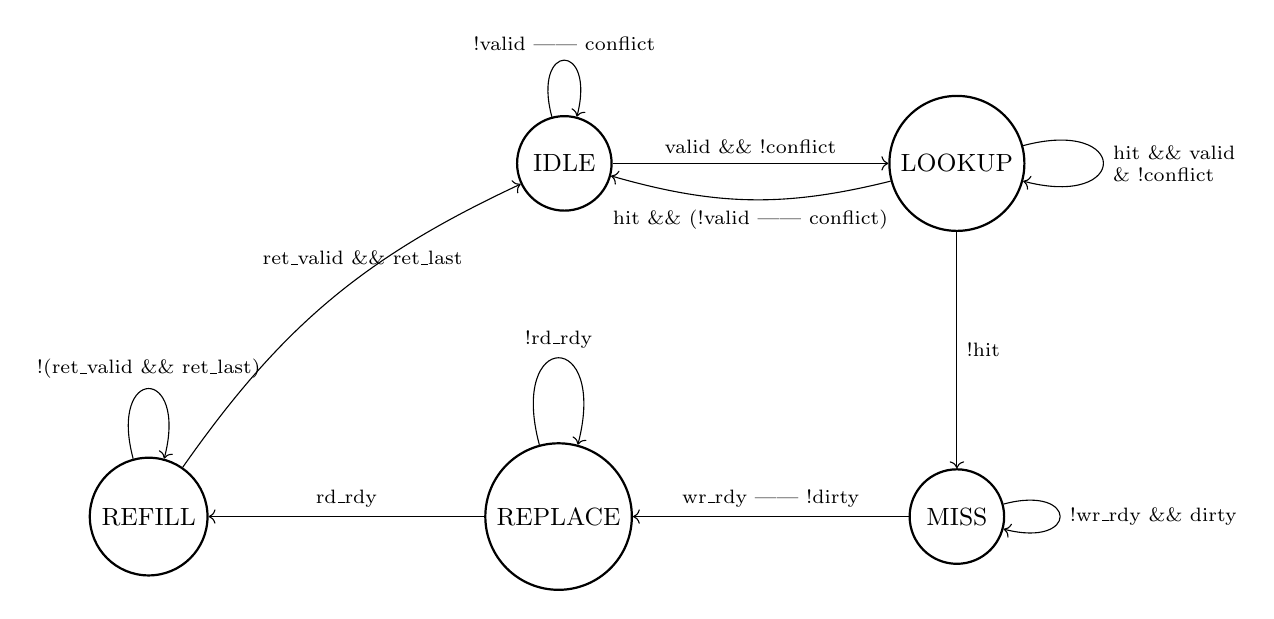
\begin{tikzpicture}[
        node distance=3cm and 3.5cm,
        state/.style={circle, draw, thick, minimum size=1.2cm, font=\small},
        every edge/.style={draw, thick, ->, >=stealth},
        every loop/.style={looseness=8}
    ]
        % Define states
        \node[state] (IDLE) {IDLE};
        \node[state, right=of IDLE] (LOOKUP) {LOOKUP};
        \node[state, below=of LOOKUP] (MISS) {MISS};
        \node[state, left=of MISS] (REPLACE) {REPLACE};
        \node[state, left=of REPLACE] (REFILL) {REFILL};
        
        % State transitions
        % IDLE -> LOOKUP
        \draw[->] (IDLE) -- node[above, font=\scriptsize] {valid \&\& !conflict} (LOOKUP);
        
        % IDLE self-loop
        \draw[->] (IDLE) to[loop above] node[above, font=\scriptsize] {!valid || conflict} (IDLE);
        
        % LOOKUP -> IDLE
        \draw[->] (LOOKUP) to[bend left=15] node[below, font=\scriptsize, pos=0.5] {hit \&\& (!valid || conflict)} (IDLE);
        
        % LOOKUP self-loop
        \draw[->] (LOOKUP) to[loop right] node[right, font=\scriptsize, align=left] {hit \&\& valid\\ \& !conflict} (LOOKUP);
        
        % LOOKUP -> MISS
        \draw[->] (LOOKUP) -- node[right, font=\scriptsize] {!hit} (MISS);
        
        % MISS -> REPLACE
        \draw[->] (MISS) -- node[above, font=\scriptsize] {wr\_rdy || !dirty} (REPLACE);
        
        % MISS self-loop
        \draw[->] (MISS) to[loop right] node[right, font=\scriptsize] {!wr\_rdy \&\& dirty} (MISS);
        
        % REPLACE -> REFILL
        \draw[->] (REPLACE) -- node[above, font=\scriptsize] {rd\_rdy} (REFILL);
        
        % REPLACE self-loop
        \draw[->] (REPLACE) to[loop above] node[above, font=\scriptsize] {!rd\_rdy} (REPLACE);
        
        % REFILL -> IDLE
        \draw[->] (REFILL) to[bend left=15] node[above, font=\scriptsize, pos=0.6] {ret\_valid \&\& ret\_last} (IDLE);
        
        % REFILL self-loop
        \draw[->] (REFILL) to[loop above] node[above, font=\scriptsize] {!(ret\_valid \&\& ret\_last)} (REFILL);
        
    \end{tikzpicture}
    \caption{Cache主状态机状态转移图}
    \label{fig:cache_fsm}
\end{figure}

在IDLE状态下,如果有新的请求到来且没有与Write Buffer冲突,状态机就会转入LOOKUP状态并将请求信息锁存到Request Buffer中。在LOOKUP状态,状态机根据Tag比较结果决定下一步动作。对于写操作命中的情况,主状态机会触发Write Buffer状态机进入WRITE状态。Write Buffer状态机的转换逻辑相对简单:

\begin{lstlisting}[language=Verilog]
always @(*) begin
    case (wb_state)
        WB_STATE_IDLE: begin
            if ((main_state == STATE_LOOKUP) && 
                (req_op == OP_WRITE) && cache_hit) begin
                wb_next_state = WB_STATE_WRITE;
            end else begin
                wb_next_state = WB_STATE_IDLE;
            end
        end
        WB_STATE_WRITE: begin
            if ((main_state == STATE_LOOKUP) && 
                (req_op == OP_WRITE) && cache_hit) begin
                wb_next_state = WB_STATE_WRITE;
            end else begin
                wb_next_state = WB_STATE_IDLE;
            end
        end
        default: begin
            wb_next_state = WB_STATE_IDLE;
        end
    endcase
end
\end{lstlisting}

如图\ref{fig:wb_fsm}所示,当主状态机在LOOKUP状态发现写命中时,Write Buffer进入WRITE状态;当没有新的写命中时,返回IDLE状态。

\begin{figure}[H]
    \centering
    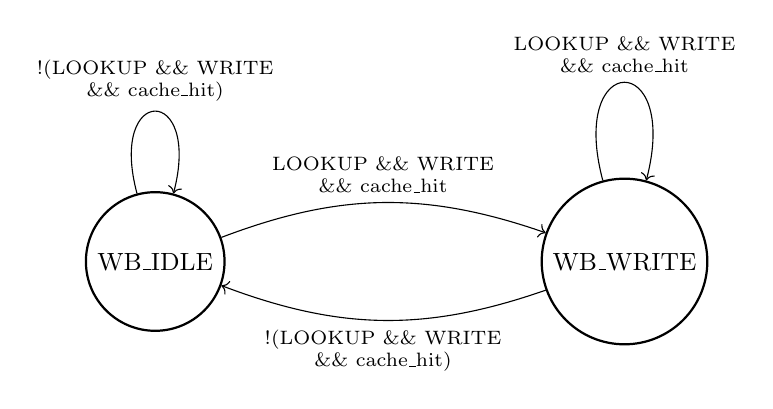
\begin{tikzpicture}[
        node distance=4cm,
        state/.style={circle, draw, thick, minimum size=1.5cm, font=\small},
        every edge/.style={draw, thick, ->, >=stealth},
        every loop/.style={looseness=8}
    ]
        % Define states
        \node[state] (IDLE) {WB\_IDLE};
        \node[state, right=of IDLE] (WRITE) {WB\_WRITE};
        
        % State transitions
        % IDLE -> WRITE
        \draw[->] (IDLE) to[bend left=20] node[above, font=\scriptsize, align=center] {LOOKUP \&\& WRITE\\ \&\& cache\_hit} (WRITE);
        
        % WRITE -> IDLE
        \draw[->] (WRITE) to[bend left=20] node[below, font=\scriptsize, align=center] {!(LOOKUP \&\& WRITE\\ \&\& cache\_hit)} (IDLE);
        
        % IDLE self-loop
        \draw[->] (IDLE) to[loop above] node[above, font=\scriptsize, align=center] {!(LOOKUP \&\& WRITE\\ \&\& cache\_hit)} (IDLE);
        
        % WRITE self-loop
        \draw[->] (WRITE) to[loop above] node[above, font=\scriptsize, align=center] {LOOKUP \&\& WRITE\\ \&\& cache\_hit} (WRITE);
        
    \end{tikzpicture}
    \caption{Write Buffer状态机状态转移图}
    \label{fig:wb_fsm}
\end{figure}

\subsubsection{Tag比较与Data选择逻辑}

Tag比较逻辑是Cache命中判断的核心。在LOOKUP状态,RAM已经读出两路的TAGV数据和Data数据。我们将TAGV RAM读出的数据拆分为Tag和Valid位,然后将每一路的Tag与Request Buffer中锁存的物理地址Tag进行相等比较。Way0命中的条件是way0\_v为1且way0\_tag等于req\_tag;Way1命中的条件是way1\_v为1且way1\_tag等于req\_tag。需要特别注意的是,对于uncache访问,即使Tag比较相等也不能认为命中,因此cache\_hit信号的生成逻辑是\texttt{(way0\_hit || way1\_hit) \&\& !req\_uncache}。这样设计能够确保uncache访问一定会走缺失处理流程,直接访问总线而不经过Cache。

\begin{lstlisting}[language=Verilog]
assign {way0_tag, way0_v} = tagv_way0_rdata;
assign {way1_tag, way1_v} = tagv_way1_rdata;
assign way0_d = dirty_way0[req_index];
assign way1_d = dirty_way1[req_index];

assign way0_hit = way0_v && (way0_tag == req_tag) && !req_uncache;
assign way1_hit = way1_v && (way1_tag == req_tag) && !req_uncache;
assign cache_hit = (way0_hit || way1_hit) && !req_uncache;
\end{lstlisting}

Data选择逻辑负责从两路Cache读出的Data中选择正确的字返回。首先,我们根据Request Buffer中锁存的offset[3:2]从每一路的128位Data(由4个Bank组成)中选择一个32位字。然后,根据Cache命中的结果从两个候选字中选择最终的返回结果。对于读操作Cache缺失的情况,最终返回的数据来自AXI总线接口的ret\_data信号。具体实现如下:

\begin{lstlisting}[language=Verilog]
// Data Select logic
wire [127:0] way0_load_block;
wire [127:0] way1_load_block;
wire [ 31:0] way0_load_word;
wire [ 31:0] way1_load_word;
wire [ 31:0] load_result;

// Concatenate 4 banks to form 128-bit block
assign way0_load_block = {data_way0_bank3_rdata, data_way0_bank2_rdata, 
                          data_way0_bank1_rdata, data_way0_bank0_rdata};
assign way1_load_block = {data_way1_bank3_rdata, data_way1_bank2_rdata, 
                          data_way1_bank1_rdata, data_way1_bank0_rdata};

// Select word from block based on offset[3:2]
assign way0_load_word = way0_load_block[req_offset[3:2] * 32 +: 32];
assign way1_load_word = way1_load_block[req_offset[3:2] * 32 +: 32];

// Final load result: way0_hit, way1_hit, or refill data
assign load_result = ({32{way0_hit}} & way0_load_word) |
                     ({32{way1_hit}} & way1_load_word) |
                     ({32{main_state == STATE_REFILL}} & ret_data);
\end{lstlisting}

这里使用了Verilog的位选择语法\texttt{[base +: width]}来从128位数据中动态选择32位字,根据offset[3:2]的值可以选择第0、1、2或3个字。最终的load\_result通过三个独热编码的选择信号进行或运算得到,确保在任何时刻只有一个数据源有效。

\subsubsection{Write Buffer与Bank冲突检测}

Write Buffer的引入是为了打断Cache RAM输出到输入的组合路径,避免时序问题。主状态机在LOOKUP状态发现写操作命中Cache时,不直接将数据写入RAM,而是先将写入信息(包括way、bank、index、写字节使能和写数据)锁存到Write Buffer中。在下一个周期,Write Buffer状态机进入WRITE状态,使用锁存的信息向Cache RAM发起写请求。这样的设计避免了Tag比较结果(来自RAM读出)直接控制Data RAM写使能的组合路径。

由于Cache采用了将Data分为4个Bank的设计,一个潜在的问题是Look Up读操作和Hit Write写操作可能同时访问同一个Bank。我们实现了冲突检测逻辑来处理这种情况:如果Write Buffer正在写入某个Bank,而新来的读请求也要访问同一个Bank(通过比较offset[3:2]和write\_bank判断),则认为发生了Bank冲突,需要阻塞新的读请求。类似地,如果主状态机在LOOKUP状态发现写命中,而新来的读请求访问相同的地址位置,也会产生冲突。这两种冲突情况都通过将addr\_ok信号置为0来阻塞流水线,等待冲突消除后再接收新请求。虽然这种阻塞方式会带来一定的性能损失,但在简单的顺序流水线中,这种损失是可以接受的,而且实现逻辑相对简单可靠。

\begin{lstlisting}[language=Verilog]
// Conflict case 1: Write Buffer is writing, and new request is 
// read operation accessing the same bank
wire conflict_case1 = (wb_state == WB_STATE_WRITE) &&
                      valid && (op == OP_READ) &&
                      (offset[3:2] == write_bank);

// Conflict case 2: Write hit detected in LOOKUP state
wire conflict_case2 = (main_state == STATE_LOOKUP) &&
                      (req_op == OP_WRITE) &&
                      valid && (op == OP_READ) &&
                      ({tag, index, offset[3:2]} == 
                       {req_tag, req_index, req_offset[3:2]});
\end{lstlisting}

\subsubsection{Request Buffer、Miss Buffer与LFSR}

Cache模块需要维护多个缓冲区来记录访问信息。Request Buffer用于锁存CPU发来的请求信息,Miss Buffer用于记录缺失处理过程中的状态,LFSR用于生成伪随机替换算法所需的随机数。

Request Buffer在主状态机接收新请求时更新,将请求的各个字段锁存下来供后续使用:

\begin{lstlisting}[language=Verilog]
// Request Buffer
reg        req_op;
reg [ 7:0] req_index;
reg [19:0] req_tag;
reg [ 3:0] req_offset;
reg [ 3:0] req_wstrb;
reg [31:0] req_wdata;
reg        req_uncache;

// Request Buffer update
always @(posedge clk) begin
    if (~resetn) begin
        req_op      <= 1'b0;
        req_index   <= 8'b0;
        req_tag     <= 20'b0;
        req_offset  <= 4'b0;
        req_wstrb   <= 4'b0;
        req_wdata   <= 32'b0;
        req_uncache <= 1'b0;
    end else if (lookup) begin
        req_op      <= op;
        req_index   <= index;
        req_tag     <= tag;
        req_offset  <= offset;
        req_wstrb   <= wstrb;
        req_wdata   <= wdata;
        req_uncache <= uncache;
    end
end
\end{lstlisting}

Miss Buffer记录缺失处理的状态,包括要替换的路号和已返回的数据计数:

\begin{lstlisting}[language=Verilog]
// Miss Buffer
reg [ 1:0] refill_word_cnt;     // Count of words returned
reg        replace_way_reg;     // Record the way to replace

// Miss Buffer update
always @(posedge clk) begin
    if (~resetn) begin
        refill_word_cnt <= 2'b0;
        replace_way_reg <= 1'b0;
    end else begin
        if (main_state == STATE_MISS && 
            main_next_state == STATE_REPLACE) begin
            replace_way_reg <= lfsr[0];  // Record random way
        end
        
        if (main_state == STATE_REPLACE && 
            main_next_state == STATE_REFILL) begin
            refill_word_cnt <= 2'b0;     // Reset counter
        end else if (main_state == STATE_REFILL && ret_valid) begin
            refill_word_cnt <= refill_word_cnt + 2'b1;  // Increment
        end
    end
end
\end{lstlisting}

LFSR(线性反馈移位寄存器)用于生成伪随机数,作为替换算法的随机源。我们使用3位LFSR,在每次完成一次Refill后更新:

\begin{lstlisting}[language=Verilog]
// LFSR (pseudo-random replacement algorithm)
reg [2:0] lfsr;
always @(posedge clk) begin
    if (~resetn) begin
        lfsr <= 3'b111;
    end else if (ret_valid && ret_last) begin
        // Linear feedback: new_bit = lfsr[1] XOR lfsr[0]
        lfsr <= {lfsr[0], lfsr[1] ^ lfsr[0], lfsr[2]};
    end
end
\end{lstlisting}

LFSR的最低位用于选择替换哪一路,通过反馈移位确保生成的序列具有良好的随机性。

\subsubsection{Replace选择与Refill数据混合}

在Cache缺失时,需要选择一个Cache行进行替换。替换逻辑使用LFSR的最低位来选择路,同时需要判断被替换的行是否为脏:

\begin{lstlisting}[language=Verilog]
// Replace selection
wire         replace_way;
wire [127:0] replace_data;
wire         replace_dirty;

assign replace_way = (main_state == STATE_MISS) ? lfsr[0] : 
                     replace_way_reg;
assign replace_data = replace_way ? way1_load_block : 
                      way0_load_block;
assign replace_dirty = (replace_way == 1'b0 && 
                        dirty_way0[req_index] && way0_v) ||
                       (replace_way == 1'b1 && 
                        dirty_way1[req_index] && way1_v);
\end{lstlisting}

在Refill阶段,如果缺失是由写操作引起的,需要将写数据与总线返回的数据混合。混合逻辑根据写字节使能选择保留哪些字节:

\begin{lstlisting}[language=Verilog]
// Refill data preparation
wire [31:0] refill_word;
wire [31:0] mixed_word;

// Mix write data and return data based on wstrb
assign mixed_word = {
    req_wstrb[3] ? req_wdata[31:24] : ret_data[31:24],
    req_wstrb[2] ? req_wdata[23:16] : ret_data[23:16],
    req_wstrb[1] ? req_wdata[15: 8] : ret_data[15: 8],
    req_wstrb[0] ? req_wdata[ 7: 0] : ret_data[ 7: 0]
};

assign refill_word = ((refill_word_cnt == req_offset[3:2]) && 
                      (req_op == OP_WRITE)) ?
                     mixed_word : ret_data;
\end{lstlisting}

这样可以确保写操作缺失时,Cache中填入的是正确混合后的数据。

\subsubsection{Dirty位管理与输出信号生成}

Dirty表需要在写命中和Refill时正确更新。在写命中时,对应的Dirty位置1;在Refill时,根据是否为写操作来设置Dirty位:

\begin{lstlisting}[language=Verilog]
// Dirty table update
always @(posedge clk) begin
    if (~resetn) begin
        dirty_way0 <= 256'b0;
        dirty_way1 <= 256'b0;
    end else begin
        if (hitwrite) begin
            if (way0_hit) begin
                dirty_way0[write_index] <= 1'b1;
            end else if (way1_hit) begin
                dirty_way1[write_index] <= 1'b1;
            end
        end else if (refill && ret_valid && 
                     (refill_word_cnt == req_offset[3:2]) && 
                     !req_uncache) begin
            if (replace_way == 1'b0) begin
                dirty_way0[req_index] <= req_op;  // 1 for write, 0 for read
            end else begin
                dirty_way1[req_index] <= req_op;
            end
        end
    end
end
\end{lstlisting}

Cache模块的输出信号根据状态和请求类型生成。addr\_ok表示能否接收新请求,data\_ok表示数据传输完成:

\begin{lstlisting}[language=Verilog]
// Cache --> CPU output signals
assign addr_ok = (main_state == STATE_IDLE) ||
                 ((main_state == STATE_LOOKUP) && cache_hit && 
                  valid && !conflict_case1 && !conflict_case2);

assign data_ok = ((main_state == STATE_LOOKUP) && 
                  (cache_hit || (req_op == OP_WRITE))) ||
                 ((main_state == STATE_REFILL) && ret_valid && 
                  ((req_uncache && (req_op == OP_READ)) ||
                   (!req_uncache && (refill_word_cnt == req_offset[3:2]) && 
                    (req_op == OP_READ))));

assign rdata = load_result;
\end{lstlisting}

对于写操作,即使Cache缺失也立即返回data\_ok,不阻塞流水线。对于uncache读操作,第一个数据返回时就置data\_ok;对于cache读操作,需要等到目标字返回时才置data\_ok。

\subsubsection{Uncache访问的处理}

对于Uncache访问,我们强制将其视为Cache缺失,复用缺失处理的数据通路。关键的区别在于读写请求的生成和RAM写使能的控制:

\begin{lstlisting}[language=Verilog]
// Cache --> AXI output signals
assign rd_req  = (main_state == STATE_REPLACE);
assign rd_type = req_uncache ? RD_TYPE_WORD : RD_TYPE_BLOCK;
assign rd_addr = req_uncache ? {req_tag, req_index, req_offset} :
                                {req_tag, req_index, 4'b0};

assign wr_req   = (main_state == STATE_MISS) && replace_dirty && 
                  !req_uncache;
assign wr_type  = WR_TYPE_BLOCK;
assign wr_addr  = replace_way ? {way1_tag, req_index, 4'b0} : 
                                {way0_tag, req_index, 4'b0};
assign wr_wstrb = 4'b1111;
assign wr_data  = replace_data;
\end{lstlisting}

在RAM写使能的生成中,需要检查req\_uncache标志,确保uncache访问不会修改Cache内容:

\begin{lstlisting}[language=Verilog]
assign tagv_way0_we = refill && (replace_way == 1'b0) && ret_valid && 
                      (refill_word_cnt == req_offset[3:2]) && 
                      !req_uncache;  // Don't write TAGV for uncache access
\end{lstlisting}

这样可以确保uncache访问正确地bypass Cache,同时最大程度地复用了已有的数据通路和控制逻辑。

\subsection{ICache集成到CPU(exp21)}

exp21的任务是将exp20完成的Cache模块作为ICache集成到CPU中,关键在于修改取指单元IFU以适配Cache接口,在总线转换桥中增加Burst传输支持,以及正确处理VIPT访问方式下的地址转换时序。

\subsubsection{IFU模块的接口修改}

IFU模块的修改是ICache集成工作的核心部分。原本IFU使用类SRAM接口与指令RAM交互,现在需要改为使用Cache接口。Cache接口采用教材中表10.2定义的信号组,包括valid、op、index、tag、offset、wstrb、wdata等输入信号,以及addr\_ok、data\_ok、rdata等输出信号。对于取指而言,操作类型始终是读(op=0),写相关的信号(wstrb和wdata)可以置为0,关键是要正确生成index、tag、offset和uncache信号。

VIPT访问方式要求使用虚拟地址的[11:4]作为index,使用物理地址的[31:12]作为tag。在IFU中,我们直接使用PC的[11:4]作为inst\_index,这是VIPT的关键特征——index来自虚拟地址,可以在地址转换完成之前就开始Cache访问。与此同时,我们将PC送入TLB进行地址转换,得到物理地址后提取其[31:12]作为inst\_tag。由于TLB查找是组合逻辑,物理地址的产生只需要一个组合路径的延迟,能够在同一个周期内与index一起送入Cache模块。这样Cache模块在下一个周期就能同时得到RAM读出的数据和物理地址tag,完成命中判断。

\begin{lstlisting}[language=Verilog]
// TLB for address translation
assign s0_vppn     = if_pc[31:13];
assign s0_va_bit12 = if_pc[12];
assign s0_asid     = csr_asid_asid;

// Physical address calculation
wire [31:0] paddr =
            csr_crmd_pg_value ?
            ( is_dmw0 ? {csr_dmw0_value[27:25], if_pc[28:0]} :
              is_dmw1 ? {csr_dmw1_value[27:25], if_pc[28:0]} :
              ( (s0_ps == 12) ?
                {s0_ppn[19:0], if_pc[11:0]} :
                {s0_ppn[19:9], if_pc[20:0]} )
             ) : if_pc;

// Instruction Cache interface
assign inst_valid   = !inst_buf_valid & !req_sent;
assign inst_op      = 1'b0;               // Always read
assign inst_index   = if_pc[11:4];        // Virtual index (VIPT)
assign inst_tag     = paddr[31:12];       // Physical tag
assign inst_offset  = if_pc[3:0];
assign inst_wstrb   = 4'b0;
assign inst_wdata   = 32'b0;
assign inst_uncache = fetch_uncache;
\end{lstlisting}

\subsubsection{Uncache访问类型的判断}

确定取指访问是否为uncache是IFU修改的另一个重要部分。根据LoongArch规范,存储访问类型由MAT(Memory Access Type)字段决定,MAT=0表示强序非缓存(SUC),MAT=1表示一致可缓存(CC)。MAT字段的来源取决于当前的地址翻译模式:在直接地址翻译模式下(DA=1, PG=0),取指的存储访问类型固定为可缓存;在直接映射窗口模式下(PG=1且DMW命中),MAT来自命中的DMW寄存器的MAT域;在页表映射模式下(PG=1且无DMW命中),MAT来自TLB查找结果的MAT域。

我们在IFU中实现了这个判断逻辑,生成fetch\_mat信号来表示当前取指的存储访问类型,然后根据fetch\_mat是否为0生成fetch\_uncache标志。这个标志随着其他Cache接口信号一起送入Cache模块,用于决定当前访问是否应该bypass Cache。需要注意的是,DMW命中判断不仅要检查地址段匹配,还要检查特权级匹配,只有当前特权级对应的PLV位为1时,才认为DMW有效。

\begin{lstlisting}[language=Verilog]
// DMW match: check both address segment and privilege level
wire dmw0_plv_ok = (csr_crmd_plv_value == 2'd0) ? csr_dmw0_value[0] : 
                   (csr_crmd_plv_value == 2'd3) ? csr_dmw0_value[3] : 1'b0;
wire dmw1_plv_ok = (csr_crmd_plv_value == 2'd0) ? csr_dmw1_value[0] : 
                   (csr_crmd_plv_value == 2'd3) ? csr_dmw1_value[3] : 1'b0;
wire is_dmw0 = dmw0_plv_ok && (if_pc[31:29] == csr_dmw0_value[31:29]);
wire is_dmw1 = dmw1_plv_ok && (if_pc[31:29] == csr_dmw1_value[31:29]);

// Determine MAT and uncache flag
wire [1:0] fetch_mat = 
            !csr_crmd_pg_value ? 2'b01 :          // DA mode: cacheable
            ( is_dmw0 ? csr_dmw0_value[5:4] :     // DMW0 MAT
              is_dmw1 ? csr_dmw1_value[5:4] :     // DMW1 MAT
              s0_mat                              // TLB MAT
            );

wire fetch_uncache = (fetch_mat == 2'b00);  // SUC (MAT=0): uncached
\end{lstlisting}

\subsubsection{IFU取指流程与异常处理}

在集成ICache后,IFU的取指流程需要考虑Cache的握手时序。我们使用inst\_buf来缓存取回的指令,使用req\_sent标志记录是否已发出请求但尚未收到数据。取指流程的核心逻辑如下:

\begin{lstlisting}[language=Verilog]
reg [31:0] if_pc;
reg [31:0] inst_buf;
reg        inst_buf_valid;
reg        req_sent;
reg        cancel;
reg [31:0] cancel_target;

always @(posedge clk) begin
    if (!resetn) begin
        if_pc          <= 32'h1c000000;
        inst_buf_valid <= 0;
        req_sent       <= 0;
        cancel         <= 0;
    end else begin
        if (!inst_buf_valid) begin
            // Buffer is empty, fetch from Cache
            if (!req_sent) begin
                if (if_ex_valid) begin
                    // Exception at IF: generate NOP instruction
                    inst_buf_valid <= 1;
                    inst_buf       <= 32'h02800000;  // NOP
                end else begin
                    req_sent <= inst_addr_ok;
                end
            end else if (inst_data_ok) begin
                // Data returned from Cache
                inst_buf <= inst_rdata;
                req_sent <= 0;
                
                if (!cancel) begin
                    inst_buf_valid <= !id_ready;
                    if (id_ready) begin
                        if_pc <= if_pc + 32'd4;
                    end
                end else if (!flush && !br_taken) begin
                    cancel <= 0;
                    if_pc <= cancel_target;
                end
            end
            
            if (flush || br_taken) begin
                // Cancel current request
                cancel        <= 1;
                cancel_target <= flush ? flush_target : br_target;
            end
        end else begin
            // Buffer is full
            if (flush || br_taken) begin
                inst_buf_valid <= 0;
                if_pc <= flush ? flush_target : br_target;
            end else if (id_ready) begin
                inst_buf_valid <= 0;
                if_pc <= if_pc + 32'd4;
            end
        end
    end
end
\end{lstlisting}

当取指发生TLB异常时,不能将无效的物理地址送到总线,而是生成一个NOP指令来携带异常信息:

\begin{lstlisting}[language=Verilog]
// Exception detection
wire        adef_error          = (if_pc[1:0] != 2'b00);
wire        tlb_gen_error       = csr_crmd_pg_value & !is_dmw0 & !is_dmw1;
wire        tlb_refill_error    = tlb_gen_error & !s0_found;
wire        fetch_invalid_error = tlb_gen_error &  s0_found & !s0_v;
wire        tlb_plv_error       = tlb_gen_error &  s0_found &  s0_v & 
                                  (csr_crmd_plv_value > s0_plv);
wire        if_ex_valid         = adef_error | tlb_refill_error |
                                  fetch_invalid_error | tlb_plv_error;
\end{lstlisting}

\subsubsection{Bridge模块的Burst传输支持}

Bridge模块的修改是exp21的另一项重要工作。我们需要支持Burst传输来优化Cache行的读取。首先在Bridge中增加Burst相关的寄存器和控制信号:

\begin{lstlisting}[language=Verilog]
reg [4:0] state;
reg [1:0] wready_buf;
reg [1:0] grant;
reg [1:0] last_grant;

// Burst transfer support
reg [2:0] burst_len;       // Number of beats in burst (0-3 for 1-4 beats)
reg [2:0] burst_cnt;       // Current beat counter
wire      is_burst;
wire      burst_finish;

assign is_burst = (grant == 2'd0) && (icache_rd_type == 3'b100);
assign burst_finish = (burst_cnt == burst_len);
\end{lstlisting}

Bridge的状态机需要处理Burst传输。在IDLE状态根据请求类型设置burst\_len,在R状态根据每次握手递增burst\_cnt:

\begin{lstlisting}[language=Verilog]
always @(posedge aclk) begin
    if (!aresetn) begin
        state      <= S_IDLE;
        wready_buf <= 2'b00;
        grant      <= 2'd0;
        last_grant <= 2'd2;
        burst_len  <= 3'd0;
        burst_cnt  <= 3'd0;
    end else begin
        case (state)
            S_IDLE: begin
                wready_buf <= 2'b00;
                burst_cnt  <= 3'd0;
                
                // Arbitration: ICache read > Data read > Data write
                if (icache_rd_req_valid) begin
                    grant <= 2'd0;
                    state <= S_AR;
                    burst_len <= (icache_rd_type == 3'b100) ? 3'd3 : 3'd0;
                end else if (data_rd_req_valid) begin
                    grant <= 2'd1;
                    state <= S_AR;
                    burst_len <= 3'd0;
                end else if (data_wr_req_valid) begin
                    grant <= 2'd2;
                    state <= S_AW;
                    burst_len <= 3'd0;
                end
            end
            
            S_AR: begin
                if (ar_hs) begin
                    state <= S_R;
                end
            end
            
            S_R: begin
                if (r_hs) begin
                    if (rlast || burst_finish) begin
                        state <= S_IDLE;
                        burst_cnt <= 3'd0;
                    end else begin
                        burst_cnt <= burst_cnt + 3'd1;
                    end
                end
            end
            
            // ... (AW and B states)
        endcase
    end
end
\end{lstlisting}

在AR通道,根据请求类型设置正确的arlen和arsize:

\begin{lstlisting}[language=Verilog]
// Request type decode for ICache
wire [7:0] icache_arlen;
wire [2:0] icache_arsize;
assign icache_arlen  = (icache_rd_type == 3'b100) ? 8'd3 : 8'd0;
assign icache_arsize = (icache_rd_type == 3'b100) ? 3'b010 :
                       (icache_rd_type == 3'b010) ? 3'b010 :
                       (icache_rd_type == 3'b001) ? 3'b001 : 3'b000;

// AR channel
assign arid    = {2'b00, grant};
assign araddr  = (grant == 2'd0) ? icache_rd_addr : data_sram_addr;
assign arlen   = (grant == 2'd0) ? icache_arlen : 8'd0;
assign arsize  = (grant == 2'd0) ? icache_arsize : {1'b0, data_sram_size};
assign arburst = 2'b01;  // INCR mode
assign arlock  = 2'b00;
assign arcache = 4'b0000;
assign arprot  = 3'b000;
assign arvalid = (state == S_AR);
\end{lstlisting}

ICache接口的输出信号生成需要正确指示Burst传输的最后一个beat:

\begin{lstlisting}[language=Verilog]
// ICache interface outputs
assign icache_rd_rdy    = (state == S_AR) && (grant == 2'd0) && arready;
assign icache_ret_valid = (state == S_R) && (grant == 2'd0) && rvalid;
assign icache_ret_last  = (state == S_R) && (grant == 2'd0) && 
                          rvalid && burst_finish;
assign icache_ret_data  = rdata;
assign icache_wr_rdy    = 1'b1;  // ICache never writes
\end{lstlisting}

Bridge还需要处理三个端口的仲裁:端口0对应ICache读请求,端口1对应Data SRAM读请求,端口2对应Data SRAM写请求。我们采用固定优先级仲裁策略,ICache读请求优先级最高,Data读次之,Data写最低。这样可以确保取指不会被数据访问阻塞,有利于流水线保持满负荷运转。对于ICache,由于没有写操作,icache\_wr\_rdy信号恒为1。

\subsection{DCache集成到CPU(exp22)}

exp22的任务是将Cache模块作为DCache集成到CPU中。

\subsection{CACOP指令支持(exp23)}

exp23的任务是在CPU中增加CACOP指令的支持。

\section{实验结果}

exp20和21成功实现了Cache模块的设计,并完成了ICache在CPU中的集成。在Cache模块级验证环境中,Cache模块通过了所有测试用例,验证了Look Up、Hit Write、Replace和Refill等基本操作的正确性。在CPU级验证中,集成了ICache的CPU成功通过了exp21对应的func测试,包括仿真和上板验证,证明了VIPT访问方式、Burst传输、Uncache处理等功能的正确性。

\section{小组成员分工}

王荦璠:负责exp20和exp21的实现。

陈琛:负责exp22的实现。

张钧玮:负责exp23的实现。


\end{document}
